\documentclass[../main.tex]
		
		\begin{document}
			\section{Equivalence Relations and Partitions}
	\begin{description}
		\item[Task:] Understand how equivalence relations divide sets.
		\item[Definition:] Let $A$ be a set. A \underline{partition} of $A$ is a collection of non empty sets, any two of which are disjoint such that their union is $A$, \textbf{i.e.} $\lambda = \{A_\alpha \mid \alpha \in I \}$ s.t. $\forall \alpha , \alpha ' \in I$ satisfy $\alpha \neq \alpha ', A_\alpha \cap A_{\alpha '} \neq \emptyset$ and $\underset{\alpha \in I}{\cup} A_\alpha = A$
		\item Here $I$ is an indexing act (may be infinite). $\underset{\alpha \in I}{A_\alpha}$ is the union of all the $A_\alpha$'s (possibly an infinite union)
		\item[Example] $\{(n, n+1) \mid n \in \mathbb{Z} \}$ is a partition of $\mathbb{R}$
		\begin{figure}[h]
			\centering
			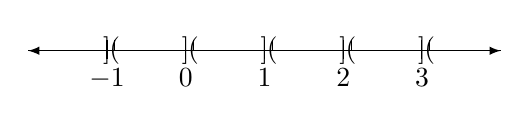
\begin{tikzpicture}
				\draw[latex-] (-2, 0) -- (4, 0);
				\draw[-latex] (-2, 0) -- (4, 0);
				
				% lines on numberline
				\foreach \x in {-1, 0, 1, 2, 3}
				\draw[shift={(\x, 0)}, color=black] (0pt, 3pt) -- (0pt, -3pt);
				
				%numbers on numberline
				\foreach \x in {-1, 0, 1, 2, 3}
				\draw[shift={(\x, 0)}, color=black] (0pt, 0pt) -- (0pt, -3pt) node[below] {$\x$};
				
				\foreach \x in {-0.9, 0.1, 1.1, 2.1, 3.1}
				\draw[shift={(\x, 0)}, color=black] (0pt, 4pt) -- (0pt, 0pt) node {{}(};
				\foreach \x in {-1, 0, 1, 2, 3}
				\draw[shift={(\x, 0)}, color=black] (0pt, 4pt) -- (0pt, 0pt) node {{}]};
			\end{tikzpicture}
		\end{figure}
		\item $\underset{n \in \mathbb{Z}}{\cup} (n, n+1 ] = \mathbb{R}$
		\item $(n, n+1 ] \cap (m, m+1 ] = \emptyset$ if $n \neq m$
		\item[Definition:] If $R$ is an equivalence relations on a set $A$ and $x \in A$, the equivalence class of $x$ denoted $[x]_R$ is the set $\{y \mid xRy \}.$ The collection of all equivalence classes is called $A$ modulo $R$ and denoted $A/R$.
		\item[Examples:]
		\begin{enumerate}
			\item[]
			\item $A = \mathbb{N} \hspace{10mm} x \equiv y$ mod 3 \\
			We have the equivalence classes $[0]_R, [1]_R$ and $[2]_R$ given by the then possible remainders under division by 3. \\
			${[0]}_R = \{0, 3, 6, 9, \dots\}$ \\
			${[1]}_R = \{1, 4, 7, 10, \dots\}$ \\
			${[2]}_R = \{2, 5, 8, 11, \dots\}$ \\
			Clearly ${[0]}_R \cup {[1]}_R \cup {[2]}_R = \mathbb{N}$ and they are mutually disjoint $\Rightarrow R$ gives a partition of $\mathbb{N}$.
			\item $ABC \sim A'B'C'$ \\
			$[ABC] = \{$The set of all triangles with angles of magnitude $\measuredangle{ABC}, \measuredangle{BAC}, \measuredangle{ACB} \}$ \\
			The union over the set of all $[ABC]$ is the set of all triangles and $[ABC] \cap [A'B'C'] = \emptyset$ if $ABC \nsim A'B'C'$ since it means these triangles have at least one angle that if difference.
			\item $A = \mathbb{C} \hspace{10mm} x \cap y$ if $|x| = |y|$ \hspace{10mm} equivalence relation \\
			$[x] = \{y \in \mathbb{C} \mid |x|=|y| \} = [r]$ for $r \in [0, +\infty) \land (r \geq 0)$ \\
			\begin{figure}[h]
				\centering
				\caption*{circle of radius $|x|$}
				\begin{tikzpicture}
					\draw(3, 0) -- (-3, 0) node[left]{Real};
					\draw(0, -3) -- (0, 3) node[above]{Imaginary};
					\draw{(0, 0)circle(2)};
				\end{tikzpicture}
			\end{figure}
			\\
			$\underset{r \in [0, +\infty)}{\cup} [r] = \mathbb{C}$ \\
			$[r_1] \cap [r_2] \neq \emptyset$ if $r_1 \neq r_2$ since two distinct circles in $\mathbb{C} \simeq \mathbb{R}^2$ with empty intersection.
			\pagebreak
			\begin{figure}[h]
				\centering
				\caption*{circles $r_1 \land r_2$}
				\begin{tikzpicture}
				\draw(-3, 0) -- (3, 0);
				\draw(0, -3) -- (0, 3);
				\draw{(0, 0)circle(2)};
				\draw{(0, 0)circle(1)};
				\end{tikzpicture}
			\end{figure}
		\end{enumerate}
		\item[Theorem:] For any equivalence relation $R$ on a set $A$, its equivalence classes form a partition of $A$, \textbf{i.e.}
		\begin{enumerate}
			\item $\forall x \in A, \exists y \in A$ s.t. $x \in [y]$ (every element of $A$ sits somewhere)
			\item $xRy \Leftrightarrow [x]=[y]$ (all elements related by $R$ belong to the same equivalence class)
			\item $\lnot (xRy) \Leftrightarrow [x] \cap [y] = \emptyset$ (if two elements are not related by $R$, the they belong to disjoint equivalence classes)
		\end{enumerate}
		\item[Proof:]
		\begin{enumerate}
			\item[]
			\item Trivial. Let $y=x$. $x \in [x]$ because $R$ is an equivalence relation. Hence reflexive, so $xRx$ holds.
			\item We will prove $xRy \Leftrightarrow [x] \subseteq [y]$ and $[y] \subseteq [x]$ \\
			$\Rightarrow$ Fix $x \in A, [x] = \{z \in A \mid xRz \} \Rightarrow \forall y \in A$ s.t. $xRy, y \in [x]$. Furthermore, $[y] = \{w \in A \mid yRw \}$ \\
			$\Rightarrow \forall w \in [u], yRw$ but $xRy \Rightarrow xRw$ by transitivity. Therefore, $w \in [x]$. We have shown $[y] \subseteq [x]$. \\
			Since $R$ is an equivalence relation, it is also symmetric. \textbf{i.e.} $xRy \Leftrightarrow yRx$. So by the same argument with $x$ and $y$ swapped $yRx \Rightarrow [x] \subseteq [y]$. Thus $xRy \Rightarrow [x] = [y]$. \\
			$\Rightarrow [x]=[y] \Rightarrow y \in [x]$ but $[x] = \{y \in A \mid xRy \}$
			\item $\Rightarrow$ We will prove the contrapositive. Assume $[x] \cap [y] \neq \emptyset \Rightarrow \exists z \in [x] \cap [y]. z \in [x]$ means $xRy$, whereas $z \in [y]$ means $yRx \Leftrightarrow zRy$ by symmetric of $R$. We thus have $xRz$ and $zRy \Rightarrow xRy$ by transitivity of $R. xRy$ contradicts $\lnot(xRy)$ so indeed $\lnot(xRy) \Rightarrow [x] \cap [y] = \emptyset$ \\
			$\Leftarrow$ Once again we use the contrapositive. \\
			Assume $\lnot(\lnot(xRy)) \Leftrightarrow xRy$. By part (b) $xRy \Rightarrow [x] = [y] \Rightarrow [x] \cap [y] \neq \emptyset$ since $x \in [x]$ and $y \in [y]$, \textbf{i.e.} These equivalence classes are non empty. We have obtained the needed contradiction.
		\end{enumerate}
		\item[qed]
		\item[Q:] What partition does "=" impose on $\mathbb{R}$?
		\item[A:] $[x]=\{x\}$ since $E = \{(x, x) \mid x \in \mathbb{R} \}$ the diagonal. \\
		The one element equivalence class is the smallest equivalence class possible (by definition, an equivalence class cannot be empty as it contains x itself). We call such a partition the \underline{finest} possible partition.
		\item[Remark:] The theorem above shows how every equivalence relations partitions a set. It turns out every partition of a set can be used to define an equivalence relation: $xRy$ is $x$ nd $y$ belong to the same subset of the partition (check this is indeed an equivalence relations!). Therefore, there is a 1-1 correspondence between partitions and equivalence relations: to each equivalence relation there corresponds a partition and vice versa.
	\end{description}
	

\end{document}